\begin{figure}[htbp]
\centering
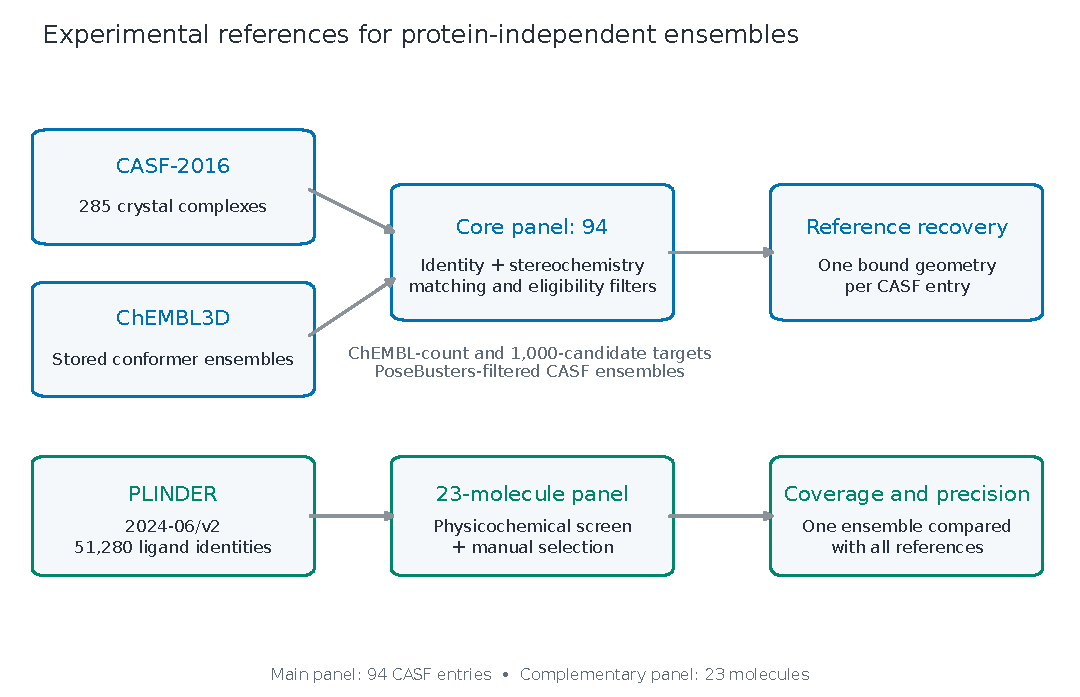
\includegraphics[width=\linewidth]{figures/experimental-panels.pdf}
\caption{Experimental evaluation panels. Matching CASF-2016 to ChEMBL3D by
molecular identity and stereochemistry, followed by eligibility filtering,
yields 94 core entries. ChEMBL3D supplies the stored comparison ensemble.
For PLINDER 2024-06/v2, physicochemical screening reduces 51,280 identities
to 25,392; ranking by distinct PDB entries and manual review yields the
23-molecule panel (Supporting Tables S5--S7). Arrows describe the evaluation
design rather than counts for individual exclusions. The larger 1,236-entry
CASF reference collection is reported in Supporting Information. PLINDER
coverage uses supplied pools without the common CASF validity filter.}
\label{fig:datasets}
\end{figure}
